% ============================================================================================================
% Optional additions to Section 2 (Background). Two blocks; neither rewords the existing text.
% ============================================================================================================

% ---- (1) Related work. Insert after the paragraph on Fisman et al. (2006) in "Data Description", before the
%          paragraph that begins "Compared to Fisman et al. ...". Each claim was checked against the papers'
%          abstracts. Bib keys Joel:2017, Eastwick:2008, Fisman:2008 are in report/references_midterm.bib.
Two later studies bear directly on our question. Joel, Eastwick and Finkel \cite{Joel:2017} ran two speed-dating
studies in which participants reported more than 100 traits and preferences beforehand, and used random forests to
predict romantic desire after each date. Their models could predict how much each person tended to desire others and
how much each person was desired, but not which particular pairs would be attracted to each other. Eastwick and
Finkel \cite{Eastwick:2008} found that the qualities people say they want in a partner before a speed-dating event fail
to predict what actually draws them to the partners they meet there. Using a speed-dating experiment by the same
authors as our data, Fisman et al.\ \cite{Fisman:2008} also studied preferences for partners of the same race, which
were stronger among women.

% ---- (2) Data figure. Insert in "Data Description" (or at the start of Section 3), after the sentence describing the
%          21 waves.
Figure~\ref{fig:events} shows that the 21 events differ greatly in size, from 25 to 484 dyads, and in how often
people matched, from 8\% to 31\%. Because the dyads of one event share people and an evening, our cross-validation
holds out whole events (Section~4).

\begin{figure}[h]
\centering
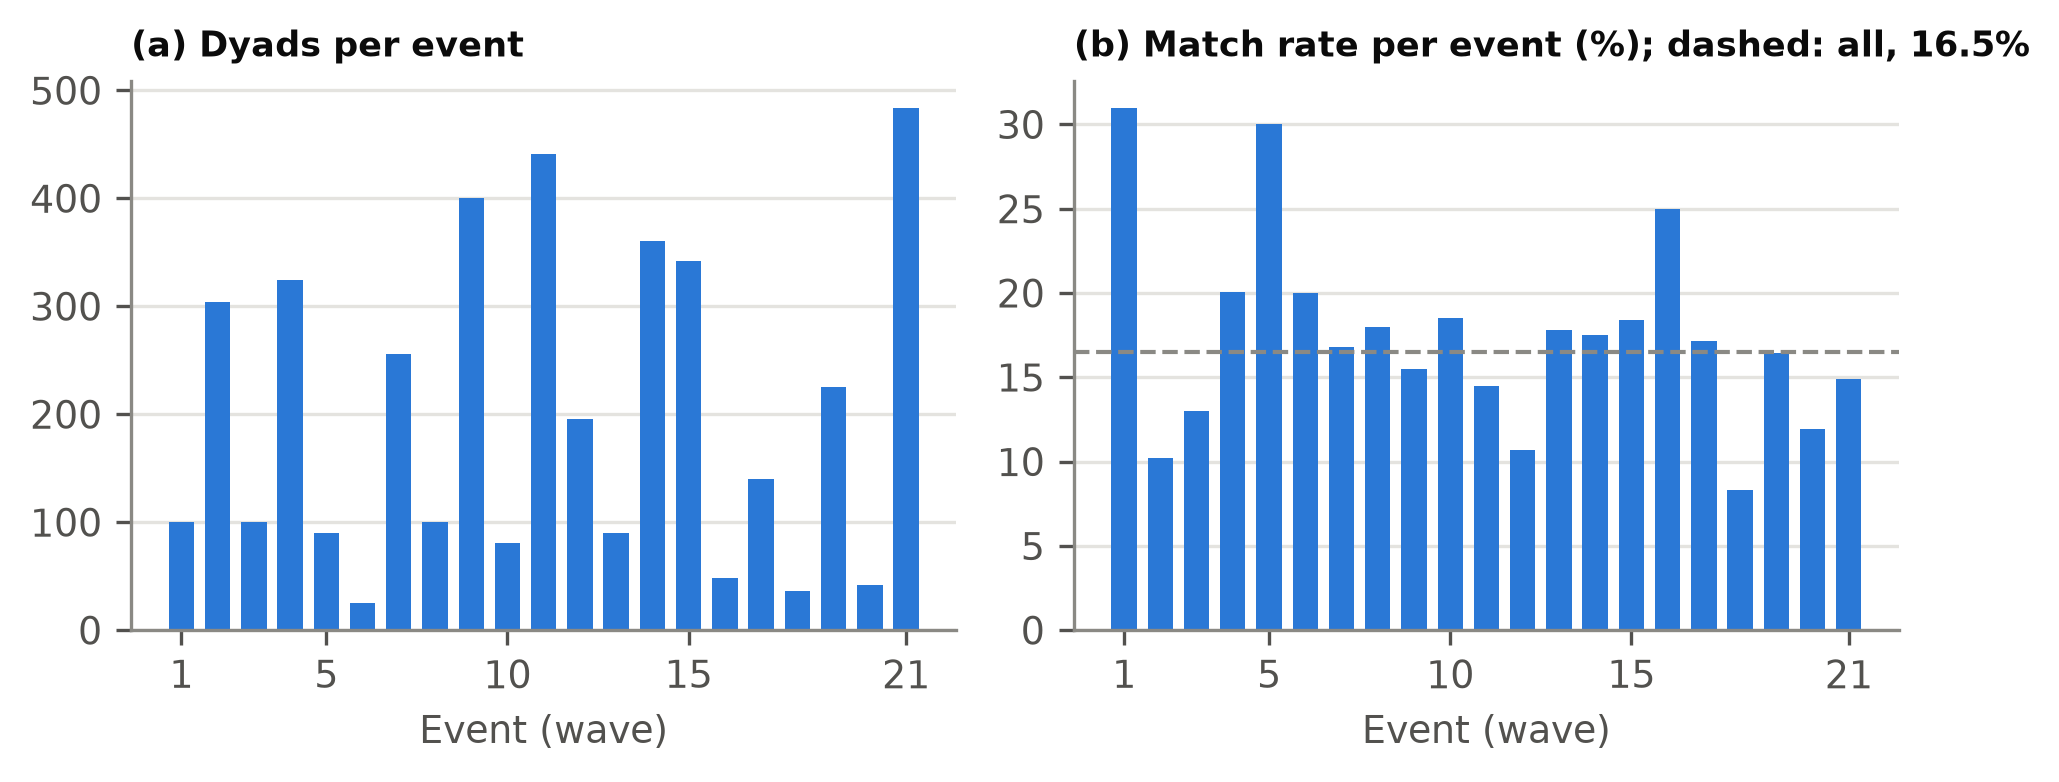
\includegraphics[width=\textwidth]{figures/paper_events.png}
\caption{Events differ in size and in how often people match. (a) Number of woman--man dyads per event; (b) match rate
per event, with the overall rate of 16.5\% dashed. Source: data/pairs.csv.}
\label{fig:events}
\end{figure}
